\section{Quaternion integration\label{quatProofs}}

Let us first consider a geometric view on quaternions, taken from~\cite{Shoemake:85}. Treat
the four components of a quaternion as Cartesian coordinates of a four-dimensional vector
space. The set of unit quaternions is then the surface of a unit hypersphere (also called a
\emph{glome}~\cite{MathWorld:4D}) in this vector space. Each point on this hypersphere
corresponds to a particular rotation. It also turns out that each pair of
opposite points on this sphere represent exactly the same rotation; hence all possible
rotations are contained in one hemisphere, no matter where the sphere is cut in half.

\subsection{Conservation of magnitude\label{quatIntegrationMagnitude}}
Define the quaternion dot product, in analogy to the 4D vector dot product, to be
\begin{equation}
\q{p}\cdot\q{q} =
    (p_w + p_x\qi + p_y\qj + p_z\qk)\cdot (q_w + q_x\qi + q_y\qj + q_z\qk) =
    p_w q_w + p_x q_x + p_y q_y + p_z q_z
\end{equation}
The dot product is commutative, contrary to the quaternion juxtaposition product.

The instantaneous rate of change is given~\cite{BaraffWitkin:97,Eberly:04,Saunders:PhD} to be
\begin{eqnarray*}
\dot{\q{q}} & = & \frac{1}{2}\tilde{\ve{\omega}}\q{q} =
    \frac{1}{2}(\omega_1\qi + \omega_2\qj + \omega_3\qk)
    (q_w + q_x\qi + q_y\qj + q_z\qk) \\*
& = & \frac{1}{2} ( - \omega_1 q_x - \omega_2 q_y - \omega_3 q_z ) +
    \frac{\qi}{2} ( \omega_1 q_w + \omega_2 q_z - \omega_3 q_y ) + \\*
&&  \frac{\qj}{2} (-\omega_1 q_z + \omega_2 q_w + \omega_3 q_x ) +
    \frac{\qk}{2} ( \omega_1 q_y - \omega_2 q_x + \omega_3 q_w )
\end{eqnarray*}

We now treat \q{q} and $\dot{\q{q}}$ as 4D vectors and calculate
their dot product:
\begin{eqnarray*}
\q{q}\cdot\dot{\q{q}} & = & \frac{1}{2} (
    - q_w \omega_1 q_x - q_w \omega_2 q_y - q_w \omega_3 q_z
    + q_x \omega_1 q_w + q_x \omega_2 q_z - q_x \omega_3 q_y \\*
&&  - q_y \omega_1 q_z + q_y \omega_2 q_w + q_y \omega_3 q_x
    + q_z \omega_1 q_y - q_z \omega_2 q_x + q_z \omega_3 q_w ) \\*
& = & 0.
\end{eqnarray*}
The rate of change is orthogonal to \q{q}, and therefore it is always
a tangent to the sphere, touching it at the point corresponding to \q{q}. The set of all possible
values of $\dot{\q{q}}$ is thus a hyperplane (a three-dimensional subspace) tangential to the
sphere at the point \q{q} in 4D space.

We can determine the magnitude $\norm{\dot{\q{q}}}$ from the sum of squares of the
components given above and find it to be
$\norm{\dot{\q{q}}} = \frac{1}{2}\norm{\ve{\omega}}\,\norm{\q{q}}$. Since we always
require $\q{q}$ to be a unit quaternion, we can reduce this to
\begin{equation}
\label{quatRateOfChangeMagnitude}
\norm{\dot{\q{q}}} = \frac{1}{2}\norm{\ve{\omega}}.
\end{equation}

Now let us determine what happens if we calculate $\q{q} + h\dot{\q{q}}$ for some finite $h$.
Note that this operation is required by all common numerical solvers of differential equations.
Consider the magnitude of the result:
\begin{eqnarray*}
\norm{\q{q} + h\dot{\q{q}}}^2 & = & (\q{q} + h\dot{\q{q}})\cdot(\q{q} + h\dot{\q{q}}) \\
&=& \q{q}\cdot\q{q} + 2h\q{q}\cdot\dot{\q{q}} + h^2\dot{\q{q}}\cdot\dot{\q{q}} \\
&=& 1 + 0 + \frac{h^2}{4}\norm{\ve{\omega}}^2 \\
&>& 1 \quad\quad\mbox{whenever}\quad \norm{\ve{\omega}} > 0.
\end{eqnarray*}

Hence, if the body in question is rotating, it is not possible for a standard numerical ODE solver
to preserve a quaternion's property of unit magnitude.


\subsection{Normalization is not enough\label{quatNormalization}}

One should think that given the derivative of a quaternion \q{q} (equation~\ref{quatRateOfChange},
page~\pageref{quatRateOfChange}), one can find $\q{q}(t + h)$ for some time step $h$ within
the accuracy of the ODE solver employed ($O(h^5)$ error for fourth-order Runge-Kutta).
Unfortunately this is not the case. This shall be demonstrated using Euler's method; it should,
however, be pointed out that more sophisticated methods like RK4 are also affected. Consider the
value of \q{q} at the next time step, $\q{q}(t + h) = \q{q}(t) + h \dot{\q{q}}(t)$. For any
non-zero $h$ and $\dot{\q{q}}$ this point will always lie outside the unit quaternion sphere due
to the orthogonality of \q{q} and $\dot{\q{q}}$. This is usually compensated by renormalizing
the quaternion after the ODE solving step. Geometrically, this renormalization can be understood
as drawing a straight line through the origin and the point $\q{q}(t) + h \dot{\q{q}}(t)$,
intersecting this line with the unit sphere and replacing $\q{q}(t + h)$ by this point of
intersection (see figure~\ref{quatNormalizationFigure}).

\begin{figure}
\psfrag{frag:q}{\q{q}}
\psfrag{frag:qdot}{$\dot{\q{q}}$}
\psfrag{frag:qplusqdot}{$\q{q} + h\dot{\q{q}}$}
\centerline{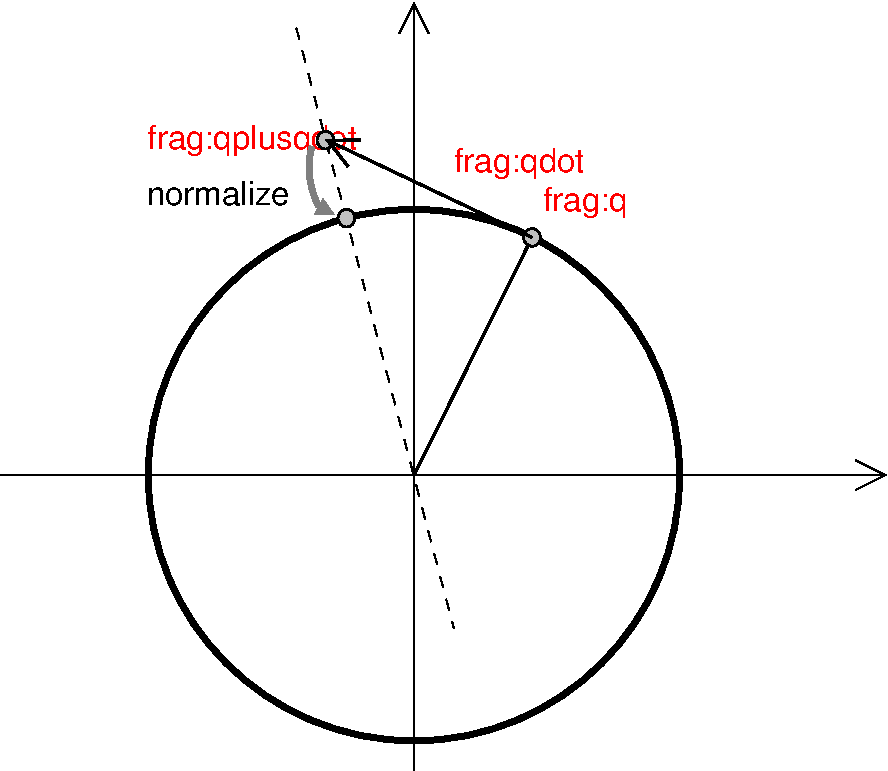
\includegraphics[width=6cm]{figures/quaternion1}}
\caption{Normalizing a quaternion after performing an ODE solving step.
    \label{quatNormalizationFigure}}
\end{figure}

Following the tangent to the sphere is a reasonable approximation to following its curve if the
magnitude of $h \dot{\q{q}}(t)$ is small compared to the curvature of the sphere.
For large time steps or large magnitudes of \ve{\omega}, however, this gets increasingly
erroneous. Consider the limiting case, a body rotating infinitely fast
($\norm{\ve{\omega}} \rightarrow \infty$): after renormalisation, $\q{q}$ will have moved merely
a quarter of the way around the unit sphere, which equates to concatenating the rotation of
quaternion \q{q} with some rotation by $180^\circ$. This is a strictly finite amount of rotation
per time step, while it would actually have been correct to perform an infinite number of
revolutions around the quaternion sphere.

If a polynomial approximation method like RK4 had been used instead of Euler's method, a parametric
polynomial space curve would have been fitted to the surface of the sphere instead of the straight
line. Note however that the Taylor series of the $\sin$ and $\cos$ functions are non-terminating,
and that it is therefore not possible for a finite polynomial curve to lie exactly in the surface
of a sphere. These ODE solvers will therefore suffer the same problems, albeit less pronounced.


\subsection{Corrected quaternion integration\label{quatIntegrationDerivation}}

Assume that the body we are simulating is rotating at a constant angular velocity.
(This assumption is later weakened by the use of a more sophisticated ODE solver,
but for now we will stick with Euler's method.) Furthermore assume without loss of
generality that the body is rotating clockwise about its $x$ axis, which corresponds
to the world's $x$ axis, and that at time $t=0$ the body's frame and the world frame
coincide. Then the orientation of the body (the quaternion describing the linear
transformation from the body's frame of reference to the world frame) is given as a
function of time by
\begin{equation}
\label{quatDerivationExact}
\q{q}(t) = \cos\left(\frac{\norm{\ve{\omega}}t}{2}\right) +
    \sin\left(\frac{\norm{\ve{\omega}}t}{2}\right)\qi
\end{equation}
(cf.\ equation~\ref{quatRotation}, figure~\ref{quatIntFig1}) and its angular velocity is
\begin{equation}
\ve{\omega} = (\omega_1, \omega_2, \omega_3)^T = (\norm{\ve{\omega}}, 0, 0)^T
\end{equation}
for some arbitrary $\norm{\ve{\omega}}$, measured in radians per unit time.

\begin{figure}
\psfrag{frag:omegat}{$\frac{\norm{\ve{\omega}} t}{2}$}
\psfrag{frag:qdotoft}{$\dot{\q{q}}(t)$}
\psfrag{frag:real}{Re}
\psfrag{frag:iimag}{$\mathsf{i}$-Im}
\centerline{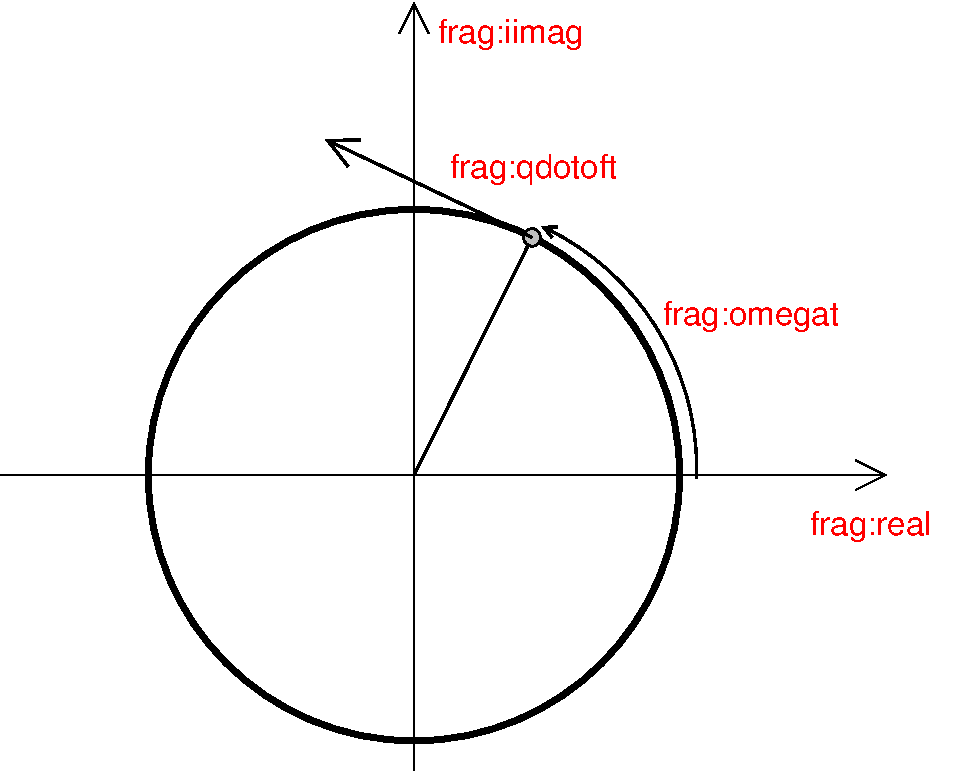
\includegraphics[width=6cm]{figures/quaternion2}}
\caption{Assumed situation for the derivation in
section~\ref{quatIntegrationDerivation}.\label{quatIntFig1}}
\end{figure}

Now assume w.l.o.g.\ that we take a time step from $t = 0$ to $t = h$.
Then we require that the result returned by Euler's method for $\q{q}(h)$
after renormalization be equal to its exact value in equation~\ref{quatDerivationExact}:
\begin{equation}
\label{quatDerivationSetup}
\cos\left(\frac{\norm{\ve{\omega}} h}{2}\right) +
    \sin\left(\frac{\norm{\ve{\omega}} h}{2}\right)\qi =
    \frac{\q{q}(0) + h \dot{\q{q}}(0)}
        {\norm{\q{q}(0) + h \dot{\q{q}}(0)}}
\end{equation}

We know from examining the 4D geometry that the value assigned to $\dot{\q{q}}$
in equation~\ref{quatRateOfChange} has the correct direction and merely needs to be
corrected in magnitude. In other words, we are searching for a scalar function
$f(h, \norm{\ve{\omega}})$ which will allow $\dot{\q{q}}$ to satisfy
equation~\ref{quatDerivationSetup}:
\begin{equation}
\dot{\q{q}}_h(t) = f\tilde{\ve{\omega}}(t)\q{q}(t)
\end{equation}

Observe that under the above assumptions $\q{q}(0) = 1$, and thus
$\dot{\q{q}}_h(0) = f \norm{\ve{\omega}} \qi$. Substituting this
into equation~\ref{quatDerivationSetup} and considering only the real part:
\begin{eqnarray*}
&& \cos\left(\frac{\norm{\ve{\omega}} h}{2}\right) =
    \left[1 + \left( f \norm{\ve{\omega}} h \right)^2 \right]^{-\frac{1}{2}} \\
&\Leftrightarrow&
    \left( f \norm{\ve{\omega}} h \right)^2 =
    \frac{1}{\cos^2\left(\frac{\norm{\ve{\omega}} h}{2}\right)} - 1 \\
&\Leftrightarrow&
    f(h, \norm{\ve{\omega}}) =
    \frac{1}{\norm{\ve{\omega}} h} \sqrt{\frac{
        1 - \cos^2\left(\frac{\norm{\ve{\omega}} h}{2}\right)}{
        \cos^2\left(\frac{\norm{\ve{\omega}} h}{2}\right)}} =
    \frac{1}{\norm{\ve{\omega}} h}
        \tan\left(\frac{\norm{\ve{\omega}} h}{2}\right)
\end{eqnarray*}

To check, we substitute this result into the $\qi$-imaginary part of
equation~\ref{quatDerivationSetup}:
\begin{eqnarray*}
\sin\left(\frac{\norm{\ve{\omega}} h}{2}\right) & = &
    \tan\left(\frac{\norm{\ve{\omega}} h}{2}\right)
    \left[ 1 + \tan^2\left(\frac{\norm{\ve{\omega}} h}{2}\right)
    \right]^{-\frac{1}{2}} \\
&=& \tan\left(\frac{\norm{\ve{\omega}} h}{2}\right)
    \left[ \frac{\cos^2\left(\frac{\norm{\ve{\omega}} h}{2}\right) +
    \sin^2\left(\frac{\norm{\ve{\omega}} h}{2}\right) }{
    \cos^2\left(\frac{\norm{\ve{\omega}} h}{2}\right) }
    \right]^{-\frac{1}{2}} \\
&=& \tan\left(\frac{\norm{\ve{\omega}} h}{2}\right)
    \cos\left(\frac{\norm{\ve{\omega}} h}{2}\right) \\
&=& \sin\left(\frac{\norm{\ve{\omega}} h}{2}\right)
\end{eqnarray*}

Thus we establish the validity of this expression for $f$. Observe that by using 
L'Hospital's rule, we can find value of $f$ for an infinitesimally small time step:
$$
\lim_{h \to 0} f = \lim_{h \to 0} \frac{ \frac{\norm{\ve{\omega}}}{2}
    \cos^{-2}\left(\frac{\norm{\ve{\omega}} h}{2}\right) }{ \norm{\ve{\omega}} } =
    \frac{1}{2}
$$
i.e.\ we obtain the original equation~\ref{quatRateOfChange} for the
instantaneous rate of change.

Now let $\Delta \q{q} = h \dot{\q{q}} =
    \frac{h}{2} \tilde{\ve{\omega}} \q{q}$.
From equation~\ref{quatRateOfChangeMagnitude} we find that
$\norm{\Delta\q{q}} = \frac{\norm{\ve{\omega}} h}{2}$.
Hence we can simplify the expression for the quaternion correcting factor by expressing it
in terms of $\Delta \q{q}$ as follows:
$$
h f \tilde{\ve{\omega}}\q{q} = \frac{h}{\norm{\ve{\omega}} h}
    \tan\left(\frac{\norm{\ve{\omega}} h}{2}\right) \tilde{\ve{\omega}} \q{q} =
    \tan\left(\norm{\Delta\q{q}}\right) \frac{\Delta\q{q}}{\norm{\Delta\q{q}}}
$$

This expression now has a clear geometric interpretation with respect to the 4D geometry
(see figure~\ref{quatIntFig2}):
$\norm{\Delta\q{q}}$ is measured in radians, and it corresponds to the \emph{correct}
angle between the old and the new vector $\q{q}$. Since $\q{q}$ and
$\dot{\q{q}}$ are orthogonal, we have a right-angled triangle between the origin,
the old and the new points $\q{q}$, and hence we can use the $\tan$ function to
evaluate the required length of the side in direction $\Delta\q{q}$.

\begin{figure}
\psfrag{frag:real}{Re}
\psfrag{frag:iimag}{$\mathsf{i}$-Im}
\psfrag{frag:q}{\q{q}}
\psfrag{frag:deltaq}{$\Delta\q{q}$}
\psfrag{frag:quergs1}{$\q{q}+\tan(\norm{\Delta\q{q}})\frac{\Delta\q{q}}{\norm{\Delta\q{q}}}$}
\psfrag{frag:quergs2}{$\mathrm{Quergs}(\q{q},\,\Delta\q{q})$}
\centerline{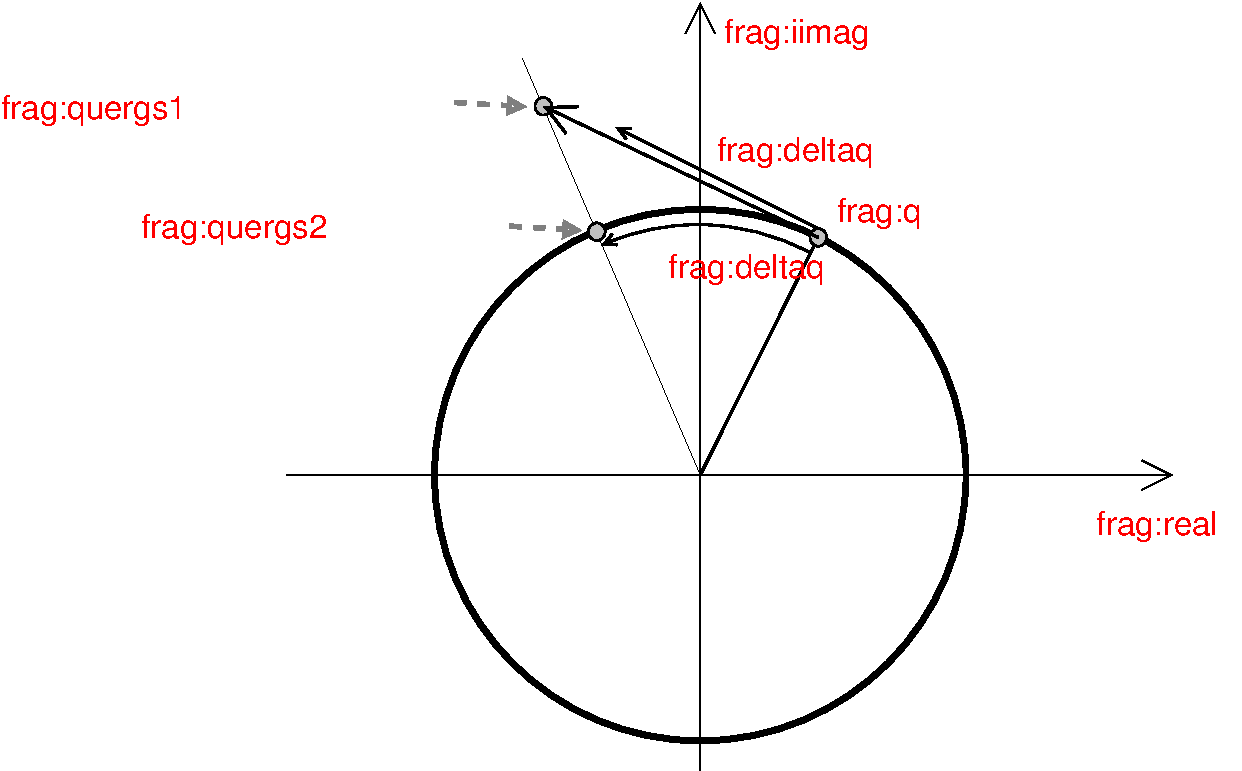
\includegraphics[width=7.7cm]{figures/quaternion3}}
\caption{Illustration of the operation of Quergs.\label{quatIntFig2}}
\end{figure}

Finally we can combine this correction and the subsequent quaternion normalisation into
a single function, which I call Quergs (for \emph{Qu}at\emph{er}nion inte\emph{g}ration
\emph{s}tep)\footnote{This naming follows the spirit of Shoemake~\cite{Shoemake:85}, whose
``Slerp'' function is an `acronym' of \emph{S}pherical \emph{l}inear int\emph{erp}olation.}:
\begin{eqnarray*}
\q{q}(t+h) = \mathrm{Quergs}(\q{q}(t), \Delta\q{q}) &=&
    \frac{\q{q}(t) + \tan\left(\norm{\Delta\q{q}}\right)
        \frac{\Delta\q{q}}{\norm{\Delta\q{q}}}}{
    \norm{\q{q}(t) + \tan\left(\norm{\Delta\q{q}}\right)
        \frac{\Delta\q{q}}{\norm{\Delta\q{q}}}}} \\
&=& \frac{\q{q}(t) + \tan\left(\norm{\Delta\q{q}}\right)
        \frac{\Delta\q{q}}{\norm{\Delta\q{q}}}}{
    \sqrt{1 + \tan^2\left(\norm{\Delta\q{q}}\right)}} \\
&=& \left[\q{q}(t) + \tan\left(\norm{\Delta\q{q}}\right)
        \frac{\Delta\q{q}}{\norm{\Delta\q{q}}}\right]
    \cos\left(\norm{\Delta\q{q}}\right)
\end{eqnarray*}
The last expression is simplest (and again allows geometric interpretation), but probably
the first of the three expressions is more useful for numerical evaluation, since it involves
only one trigonometric function and minimizes numerical errors.

When implementing this formula, care must be taken around the discontinuities of the $\tan$
function, where numerical instability may occur. These discontinuities are reached whenever a
body performs an odd multiple of half revolutions during a single time step.
